\chapter{Desarrollo}
\label{cap:desarrollo}

En este capítulo se va a llevar a cabo el estudio del arte relativo a este proyecto y se van a comentar el proceso realizado para conseguir los objetivos establecidos.

\section{Estudio del arte}

El estudio del arte debe hacerse por partida doble. Debe estudiarse el estado en el que se encuentra Android y a parte, los \texit{CBIR} en dicha plataforma.\\

\subsection{Estado arte Android}

Por la parte de la lógica no hay ningún tipo de misterio, ya que tratamos con Java y XML, cosas que apenas cambian y ya se tienen muy estudiadas e asimiladas, por lo que no es necesario un gran estudio de esta parte.\\

Lo que si hay que tener en cuenta es el desarrollo de interfaces de usuario. Este es un tema muy importante, ya que aunque la aplicación funcione correctamente y presente unas novedades increibles, un mal diseño de interfaz puede provocar su abando por parte de los usuarios. Resulta natural dedicar un tiempo de investigación a esta parte.\\

\subsubsection{Material design}
Al realizar cualquier búsqueda sobre diseño de interfaces en Android nos encontramos con \textit{Material design}, que se trata de una guía integral para el diseño visual, de movimientos y de interacción en distintas plataformas y dispositivos. Presenta una gran serie de nuevos elementos y novedades. Actualmente es el estándar de Android. Debido a esto, se debe seguir \textit{Material design} a la hora de realizar una interfaz.

\begin{figure}[H] %con el [H] le obligamos a situar aquí la figura
\centering
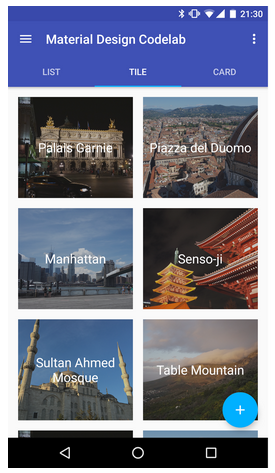
\includegraphics[scale=0.5]{imagenes/desing1.png}  %el parámetro scale permite agrandar o achicar la imagen. En el nombre de archivo puede especificar directorios
\label{design1}
\caption{Ejemplo de Material Design 1}
\end{figure}

\begin{figure}[H] %con el [H] le obligamos a situar aquí la figura
\centering
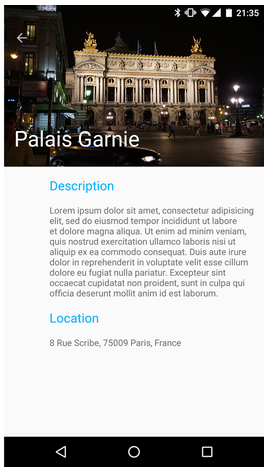
\includegraphics[scale=0.5]{imagenes/desing2.png}  %el parámetro scale permite agrandar o achicar la imagen. En el nombre de archivo puede especificar directorios
\label{design1}
\caption{Ejemplo de Material Design 2}
\end{figure}

Tras un estudio preliminar de \textit{Material design} se procedió a estudiar con más detalle dos elementos. Estos son \textit{floating action button}, \textit{Bottom Navigation} y \textit{Glide}.

\subsubsection{Floating action button}

Un \textit{Floating action button} representa la acción principal en una aplicación. Normalmente se encuentra en forma de un icono en cicular que se encuentra flotando sobre la interfaz de usuario, cambia de color al pulsar y se eleva al seleccionar. Cuando se presiona, puede contener más acciones relacionadas.\\

En mi caso he utilizado la implementación usada por \textit{Clans}, el código fuente se puede encontrar en su \href{https://github.com/Clans/FloatingActionButton}{repositorio}

\begin{figure}[H] %con el [H] le obligamos a situar aquí la figura
\centering
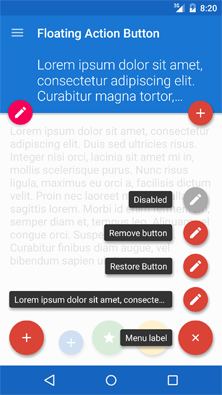
\includegraphics[scale=0.5]{imagenes/fab.png}  %el parámetro scale permite agrandar o achicar la imagen. En el nombre de archivo puede especificar directorios
\label{fab}
\caption{Ejemplo Floating action button}
\end{figure}

\subsubsection{Bottom Navigation}

Los \textit{Bottom Navigation} nos proporciona una navegación rápida entre las vistas de nivel superior de una aplicación. Está diseñado principalmente para su uso en dispositivos móviles. Las pantallas más grandes, como el escritorio, pueden lograr un efecto similar usando la navegación lateral. Por ejemplo, el tratamiento compacto "rail" muestra los iconos de navegación de forma predeterminada.\\

En mi caso he utilizado la implementación usada por \textit{sephiroth74}, el código fuente se puede encontrar en su \href{https://github.com/sephiroth74/Material-BottomNavigation}{repositorio}\\

\begin{figure}[H] %con el [H] le obligamos a situar aquí la figura
\centering
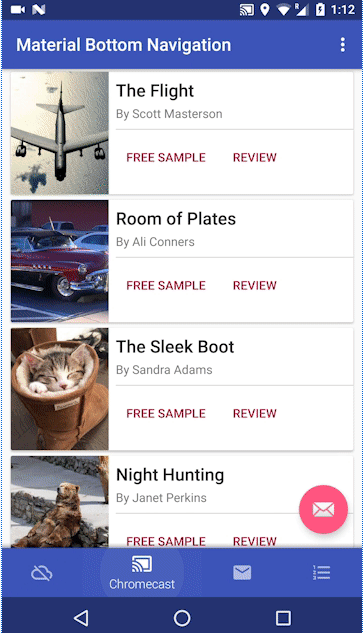
\includegraphics[scale=0.5]{imagenes/mbottom.png}  %el parámetro scale permite agrandar o achicar la imagen. En el nombre de archivo puede especificar directorios
\label{mbottom}
\caption{Ejemplo Bottom Navigation}
\end{figure}

\subsubsection{Glide}

Se trata de un marco de trabajo rápido y eficiente de código abierto que se encarga de la gestión de imágenes, agrupando la decodificación de medios, la gestión de memoria y el almacenamiento de cache en disco mediante una interfaz simple y sencilla de utilizar.\\

Actualmente se encuentra recomendada por \textit{Google}, está desarrollada por \textit{Bump Technologies}, y se puede consultar en el enlace de su \href{https://github.com/bumptech/glide}{repositorio}\\


\begin{figure}[H] %con el [H] le obligamos a situar aquí la figura
\centering
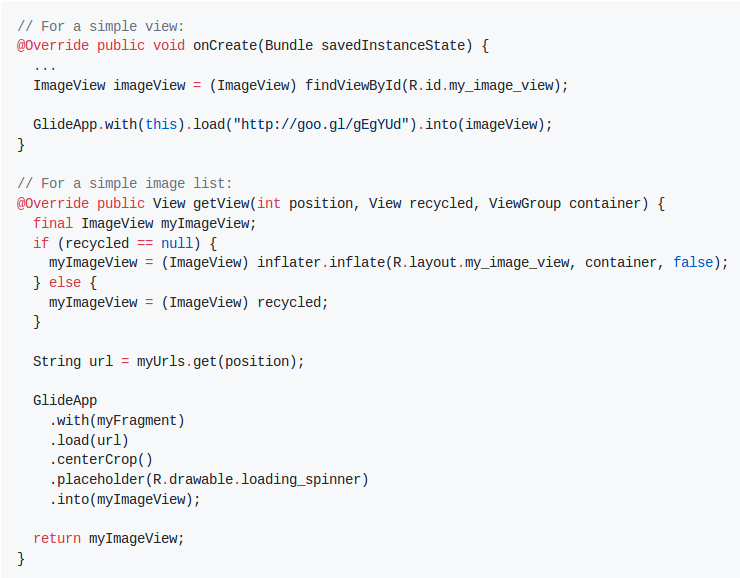
\includegraphics[scale=0.5]{imagenes/glide.png}  %el parámetro scale permite agrandar o achicar la imagen. En el nombre de archivo puede especificar directorios
\label{glide}
\caption{Ejemplo de uso de Glide}
\end{figure}

En nuestro caso es ideal, ya que nos proporciona una manera sencilla de trabajar con imágenes y a su vez, nos permite utilizar movimientos de desplazamiento scroll de una manera simple, lo que nos posibilita centrarnos en la manera en la que queremos representar las imágenes.

\subsection{Estado CBIR Android}

Lo primero que podemos encontrar es información abundante sobre CBIR en computadores, pero en nuestro caso no nos es necesaria, ya que partimos de uno previo, Java Multimedia Retrival, que cuenta con todo lo que necesitamos sobre este tipo de sistemas. Aunque siempre es interesante estar al día en estos asuntos.\\

Por lo que vamos a centrarnos en los CBIR desarrollados exclusivamente para sistemas Android.

\subsubsection{Content based image retrieval using color and texture feature extraction in Android}

Se trata de un artículo escrito por \textit{M Vel Murugan} y \textit{P Jeyanthi}, del departamento de tecnologías de la información de la universidad de Sathyabama, Chennai, Tamil Nadu.\\

En el comentan que técnicas utilizan, como la extracción de características del color se hace por el método del refinamiento del histograma del color y la extracción de la característica de textura es adquirida por la matriz de la coinocceso del nivel del gris (GLCM), es decir, estos serían sus descriptores.


\subsubsection{Content based image retrieval for mobile systems}

En esta ocasión nos encontramos ante un artículo escrito por \textit{P Jeyanthi} profesor asociado del departamento de tecnologías de la información de la universidad Sathyabama, Rajiv Gandhi Salai, India.\\

En el artículo se habla sobre un enfoque para la realización de la extracción de características basadas en textura por la co-ocurrencia de nivel de gris y la matriz de color basado en la extracción de características por color vector de concurrencia. La mayor parte del artículo se centra en el cálculo de descriptores, cosa que como se ha mencionado antes, a nosotros no nos es relevante. Por otro lado podemos ver un poco de la interfaz, lo que si nos interesa, aunque comprobamos de que se trata de una interfaz muy pobre, ya que se concentran en el cálculo de descriptores más que en la representación de los resultados.


\begin{figure}[H] %con el [H] le obligamos a situar aquí la figura
\centering
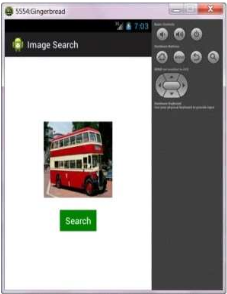
\includegraphics[scale=0.6]{imagenes/articulo11.png}  %el parámetro scale permite agrandar o achicar la imagen. En el nombre de archivo puede especificar directorios
\label{articulo11}
\caption{Interfaz CBIR for mobile systems 1}
\end{figure}

\begin{figure}[H] %con el [H] le obligamos a situar aquí la figura
\centering
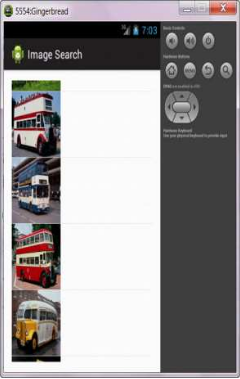
\includegraphics[scale=0.6]{imagenes/articulo12.png}  %el parámetro scale permite agrandar o achicar la imagen. En el nombre de archivo puede especificar directorios
\label{articulo11}
\caption{Interfaz CBIR for mobile systems 2}
\end{figure}

Otro de los aspectos que nos interesan es el tiempo de cómputo y el consumo de recursos, pero no se hace ningún tipo de referencia a estos aspectos en el artículo.\\

Tras realizar un estudio del estado del arte de los CBIR en Android podemos llegar a la conclusión de que se tratan de sistemas que han sido poco explotados en dicha plataforma, y lo más importante, el usuario medio no conoce de su existencia, por lo que este proyecto cubre un espacio de mercado que se encuentra desocupado.\\

\section{Proceso de desarrollo}

En esta sección vamos a detallar los distintos elementos que componen el proyecto con un nivel de detalle suficiente para dar una visión global del proyecto y entender cada uno de sus componentes.\\








